\section{Challenges with Parallel Programs}
\label{sec:challenges with parallel programs}

Parallel computing has a number of challenges related to concurrency such as deadlock and race conditions, which we will discuss in this section.

As depicted in \cref{fig:parallel patterns} we will consider three different cases of challenges with parallel programming: The map, the gather and the scatter operation.
The map operation is a trivial parallel algorithm which do not pose any parallel challenges.
Often map operations will have fast parallel implementations as we will show in \cref{sec:map} and \cref{sec:transpose}.
The gather operation is more difficult to handle as it has race conditions because it is a many-to-one operation, which we also present in \cref{sec:reduce} and \cref{sec:histogram}.
The scatter operation also suffers from challenges with race conditions such as shown in \cref{sec:scan}.

\begin{figure}[htb]
  \centering
  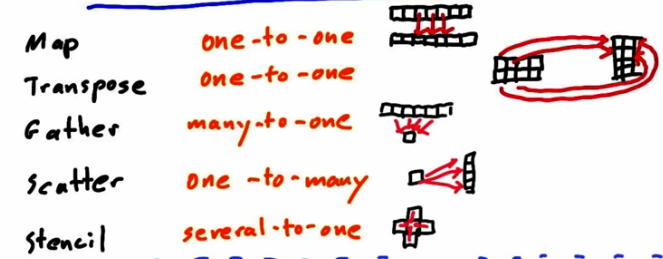
\includegraphics[width=.7\textwidth]{images/parallel-communication.png}
  \caption{Parallel communication patterns}
  \label{fig:parallel patterns}
\end{figure}

A program is in a deadlocked state if two or more threads are waiting for the other to finish, resulting in neither ever finishing.
This results in a program that will never advance and is thus considered being in a ``deadlock''.
A race condition is a situation where two or more threads attempt to perform two or more operations at the same time, where these operations must be performed in a proper order to be correct.
For instance, simultaneous update operations to the same memory address will cause a race condition.~\cite{farber2011cuda}

To give an example on how a race condition arises we present a naive implementation of a histogram in \cref{lst:naive histo}.
In the naive histogram we have no guarantee that the value of \ttt{d\_bins} have not changed between reading the value at line 9 and writing to it at line 10.
With no guarantee of having a correct representation of the bin, the thread might make an unintended write to the array as many other threads could have tried to increment in between.
In order to handle this race condition we need to utilize the synchronization tools given through CUDA.

\begin{lstlisting}[caption={Naive histogram implementation with race condition}, label={lst:naive histo}]
__global__
void naive_histogram_kernel(int *d_bins, const int *d_in, const int SIZE) {
  int tid  = threadIdx.x + blockDim.x * blockIdx.x;
  // fetch item from input
  int item = d_in[tid];
  // compute where to put item wrt. bin count
  int bin  = item % SIZE;
  // update amount for that bin
  current_value = d_bins[bin];
  d_bins[bin] = current_value + 1;
  // atomicAdd(&(d_bins[bin]), 1);
}
\end{lstlisting}

One solution to this problem is to use the atomic function where the given memory is locked while a thread is updating it and unlocked when the thread has completed the update.
By replacing line 9 and 10 with line 11 the kernel will execute an atomic operation.
The atomic operation has a slight overhead, but the cost is small~\cite{udacity}.
The issue with using atomic is that it will force a serial access to a memory slot.
In the worst case, when size of bin is one, the GPGPU is forced to act in a serial manner.
